Considering the limitations outlined in section
\ref{sssec:mapreduce_limitations}, Vinod Kumar Vavilapalli et
al. presented YARN \cite{Vavilapalli:2013:AHY:2523616.2523633} the new
resource management layer that was adopted in Hadoop 2.0. The new
Hadoop stack now is depicted in Figure \ref{fig:yarn_hadoop1_hadoop2_arch} where YARN is the
cluster resource management module and MapReduce is one out of plenty
applications running on top of YARN. This architectural transformation
paved the way for a wide variety of frameworks like
Apache Spark \cite{apache_spark}, Apache Flink \cite{apache_flink},
Apache Pig \cite{apache_pig}, etc to run on the
Hadoop platform like any other YARN application.

\begin{figure}
\centering
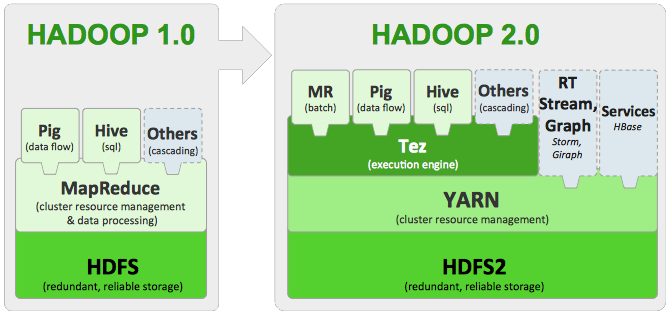
\includegraphics[scale=0.6]{resources/images/Background/hadoop1_hadoop2_arch.png}
\label{fig:yarn_hadoop1_hadoop2_arch}
\caption{Hadoop 2.0 stack \cite{hortonworks_hadoop_stack}}
\end{figure}

The new architecture of Hadoop 2.x separates the resource management
functions from the programming model. It delegates the
intra-application communication and the tracking of the execution flow
to per-job components. That unlocks great performance improvements,
improves scalability and enables a wide variery of frameworks to share
the cluster resources in a very gentle way.

YARN uses three main components to provide a scalable and fault
tolerant resource management platform. The first component is the
\emph{ResourceManager} (RM), a per-cluster daemon that tracks resource
usage and node liveness and schedules jobs on the cluster. The second
component is a per-node \emph{NodeManager} (NM) which is responsible
for monitoring resource availability on the specific node, reporting
faults to RM and managing container lifecycle. Finally, there is the
\emph{ApplicationMaster} (AM) which coordinates the logical plan of a
single job, manages the physical resources offered by the RM and
tracks the execution of the job. A high level overview of YARN
architecture is described in Figure \ref{fig:yarn_arch_overview}. RM
has a global view of the cluster and provides the scheduling
functionality, while the per-job AM manages the dynamic resource
requests and the workflow of the tasks. Containers that are allocated
by the RM are locally managed by the NM in each node in the cluster.

\begin{figure}
\centering
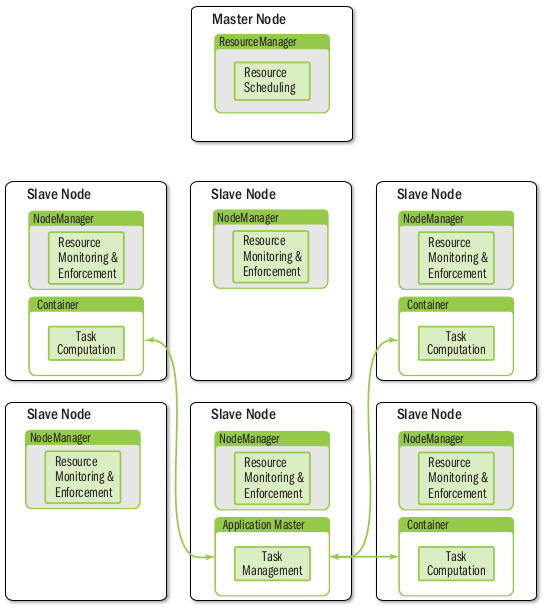
\includegraphics[scale=0.5]{resources/images/Background/yarn_arch_overview.png}
\label{fig:yarn_arch_overview}
\caption{YARN architecture overview \cite{Murthy:2014:AHY:2636998}}
\end{figure}

\subsubsection{ResourceManager}
\label{sssec:rm}
In YARN the RM acts as the central authority for allocating resources
in the cluster. It works closely with the per-node NodeManager getting
an updated view of the cluster by the heartbeats received. The RM
itself allocates generic resources in the cluster in the form of
\emph{containers} that have specific CPU and RAM requirements. Those
resource requests are piggybacked in the heartbeats issued by every AM.
As RM is completely unaware about the job execution plan,
it is up to the AM to make local optimizations and assign the
resources accordingly. RM internally consists of several modules but
the three most important are the \emph{ApplicationMasterService}, the
\emph{ResourceTrackerService} and the \emph{Yarn Scheduler} as shown
in Figure \ref{fig:yarn_RM_components}.

\begin{figure}
\centering
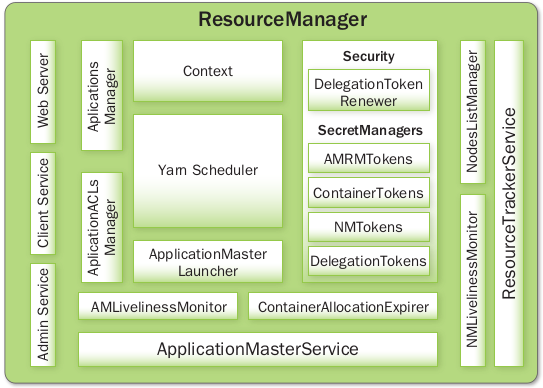
\includegraphics[scale=0.5]{resources/images/Background/RM_components.png}
\label{fig:yarn_RM_components}
\caption{ResourceManager components}
\end{figure}

The \emph{ApplicationMasterService} is responsible for receiving and
handling heartbeats from the AMs that are launched in the
cluster. Heartbeats are designed to be as compact as possible, still
not excluding any vital information. For that reason, Google Protocol
Buffers \cite{proto_buf} are used for every communication among YARN
components. Protocol Buffers is a language-neutral, platform-neutral
mechanism for efficiently serializing data. The heartbeat mechanism
serves both as a scalable way for the RM and AM to communicate, but
also for the RM to track the liveness of AMs. \emph{ResourceRequests}
contain information such as the resources per container in terms of
virual cores and memory, the number of containers, locality
preferences and priority of requests. The scheduler then tracks,
updates and satisfies these requests with available resources in the
cluster. The RM builds the view of the cluster with the available
resources from the information it receives from the NMs. The scheduler
tries to match the locality constraints as much as possible and
responds back to AM with the allocated containers along with
credentials that grant access to them. The RM also keeps track of the
AM health through the heartbeats received. The component that handle
the liveness property of every AM is the \emph{AMLivenessMonitor}. In
case of a missed heartbeat, then that particular AM is deemed dead and
is expired by the RM. All the containers that were allocated for
that AM are marked as dead and the RM reschedules the same application
(ApplicationMaster) on a new container.

\subsubsection{ApplicationMaster}
\label{sssec:am}
ApplicationMaster stuff...

\subsubsection{NodeManager}
\label{sssec:nm}
NodeManager stuff...

\subsubsection{YARN HA \& fault tolerance}
\label{sssec:yarn_ha}
YARN HA and fault tolerance stuff...
